\documentclass{standalone}

\usepackage{pgfplots}
\pgfplotsset{compat=newest}

\begin{document}
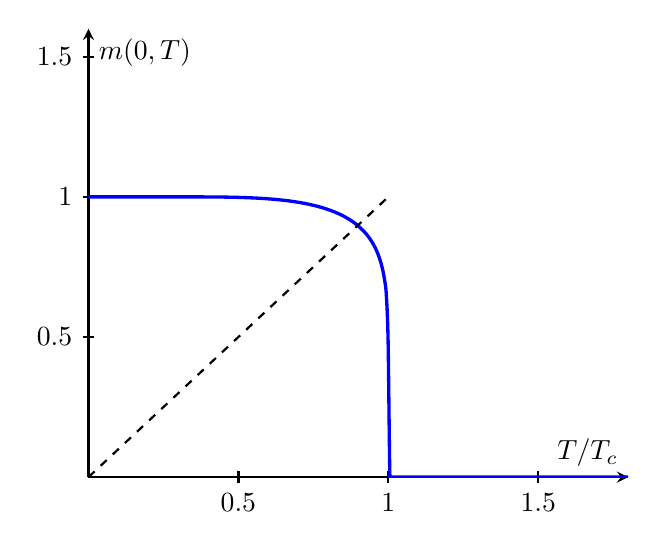
\begin{tikzpicture}[
    declare function={
        % arcsinh
        arcsinh(\x) = ln(\x + sqrt(\x^2+1));
        % magnetization
        m(\x) = and(\x>=0,\x<1) * (1 - (sinh(arcsinh(1)/x))^(-4))^(1/8) + or(\x<0,\x>=1) * (0);
      }]

  \begin{axis}[
      xlabel = {$T/T_c$},
      ylabel = {$m(0,T)$},
      smooth,thick,
      domain=0:1.8,
      ymax=1.6,
      axis lines = center,
      every tick/.style = {thick}]

    \addplot[color=blue,very thick,samples=300]{m(x)};
    \addplot[color=black,dashed,domain=0:1]{x};

  \end{axis}
\end{tikzpicture}
\end{document}
